\documentclass[usenames,dvipsnames,tikz]{standalone}
\usetikzlibrary{shapes.geometric}
\usepackage{xcolor}
\colorlet{tBlue}{RoyalBlue!35!Cerulean}
\colorlet{tRed}{Red}
\definecolor{tGreen}{HTML}{569909}
\definecolor{tOrange}{HTML}{FA7602}
\usepackage{tikz}
\usepackage{standalone}
\usepackage{amsmath}
\usepackage{mathtools}
\begin{document}	
	
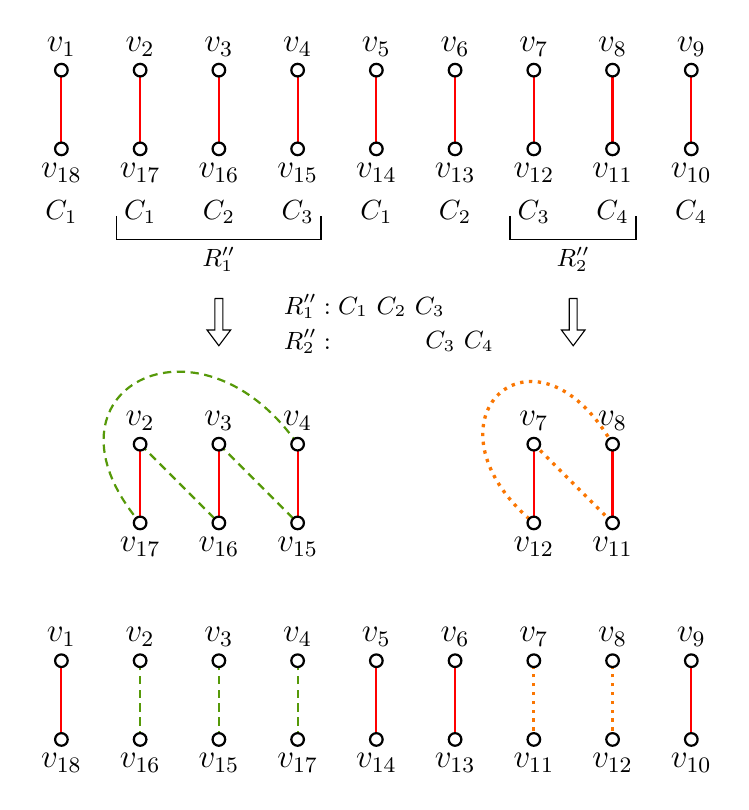
\begin{tikzpicture}
%\draw [help lines] (-1,-1) grid (10, 10);

% LIST OF EDGES FOR BCR.
\draw [thick, tRed] (1,7.5) -- (1,8.5);
\draw [thick, tRed] (2,7.5) -- (2,8.5);
\draw [thick, tRed] (3,7.5) -- (3,8.5);
\draw [thick, tRed] (4,7.5) -- (4,8.5);
\draw [thick, tRed] (5,7.5) -- (5,8.5);
\draw [thick, tRed] (6,7.5) -- (6,8.5);
\draw [thick, tRed] (7,7.5) -- (7,8.5);
\draw [thick, tRed] (8,7.5) -- (8,8.5);
\draw [thick, tRed] (9,7.5) -- (9,8.5);

\draw [fill=white, thick] (1,7.5) circle [radius = 0.08];
\draw [fill=white, thick] (2,7.5) circle [radius = 0.08];
\draw [fill=white, thick] (3,7.5) circle [radius = 0.08];
\draw [fill=white, thick] (4,7.5) circle [radius = 0.08];
\draw [fill=white, thick] (5,7.5) circle [radius = 0.08];
\draw [fill=white, thick] (6,7.5) circle [radius = 0.08];
\draw [fill=white, thick] (7,7.5) circle [radius = 0.08];
\draw [fill=white, thick] (8,7.5) circle [radius = 0.08];
\draw [fill=white, thick] (9,7.5) circle [radius = 0.08];

\draw [fill=white, thick] (1,8.5) circle [radius = 0.08];
\draw [fill=white, thick] (2,8.5) circle [radius = 0.08];
\draw [fill=white, thick] (3,8.5) circle [radius = 0.08];
\draw [fill=white, thick] (4,8.5) circle [radius = 0.08];
\draw [fill=white, thick] (5,8.5) circle [radius = 0.08];
\draw [fill=white, thick] (6,8.5) circle [radius = 0.08];
\draw [fill=white, thick] (7,8.5) circle [radius = 0.08];
\draw [fill=white, thick] (8,8.5) circle [radius = 0.08];
\draw [fill=white, thick] (9,8.5) circle [radius = 0.08];

\node at (1,7.2) {\large{$v_{18}$}};
\node at (2,7.2) {\large{$v_{17}$}};
\node at (3,7.2) {\large{$v_{16}$}};
\node at (4,7.2) {\large{$v_{15}$}};
\node at (5,7.2) {\large{$v_{14}$}};
\node at (6,7.2) {\large{$v_{13}$}};
\node at (7,7.2) {\large{$v_{12}$}};
\node at (8,7.2) {\large{$v_{11}$}};
\node at (9,7.2) {\large{$v_{10}$}};

\node at (1,8.8) {\large{$v_1$}};
\node at (2,8.8) {\large{$v_2$}};
\node at (3,8.8) {\large{$v_3$}};
\node at (4,8.8) {\large{$v_4$}};
\node at (5,8.8) {\large{$v_5$}};
\node at (6,8.8) {\large{$v_6$}};
\node at (7,8.8) {\large{$v_7$}};
\node at (8,8.8) {\large{$v_8$}};
\node at (9,8.8) {\large{$v_9$}};

\node at (1,6.7) {$C_1$};
\node at (2,6.7) {$C_1$};
\node at (3,6.7) {$C_2$};
\node at (4,6.7) {$C_3$};
\node at (5,6.7) {$C_1$};
\node at (6,6.7) {$C_2$};
\node at (7,6.7) {$C_3$};
\node at (8,6.7) {$C_4$};
\node at (9,6.7) {$C_4$};

\draw [semithick] (1.7,6.65) -- (1.7,6.35) -- (4.3,6.35) -- (4.3,6.65);
\draw [semithick] (6.7,6.65) -- (6.7,6.35) -- (8.3,6.35) -- (8.3,6.65);

%\node at (3,6.1) {\small{$R^*_1$}}; % R^*
%\node at (7.5,6.1) {\small{$R^*_2$}}; % R^*

\node at (3,6.1) {\small{$R''_1$}}; % R''
\node at (7.5,6.1) {\small{$R''_2$}}; % R''

%\node at (5.25,5.3) {\small{$\mathcal{R}^* = \{R^*_1, R^*_2\}$}};
%\node [right] at (3.7,5.5) {\small{$R^*_1: C_1, C_2, C_3$}}; % R^*
%\node [right] at (3.7,5.1) {\small{$R^*_2:$}}; % R^*
%\node [right] at (3.7,5.5) {\small{$R''_1: C_1, C_2, C_3$}}; % R''
%\node [right] at (3.7,5.1) {\small{$R''_2:$}}; % R''
%\node [right] at (5.44,5.1) {\small{$C_3, C_4$}};

\node [right] at (3.7,5.5) {\small{$R''_1: C_1\text{ }C_2\text{ }C_3$}}; % R''
\node [right] at (3.7,5.05) {\small{$R''_2:$}}; % R''
%\node [right] at (5.3675,5.05) {\small{$C_3\text{ }C_4$}};
\node [right] at (5.5,5.05) {\small{$C_3\text{ }C_4$}};
%\draw [semithick, tRed] (5.45, 5) -- (5.45, 4.85) -- (5.9, 4.85) -- (5.9, 5);
%\draw [tRed] (5.43, 4.85) rectangle (5.9, 5.725);


%----------------------------------------------------------------
% R1
%\node at (3,5.3) {\small{$R^*_1$}};
\draw (2.95,5.6) -- (2.95, 5.2) -- (2.85,5.2) -- (3,5) -- (3.15,5.2) -- (3.05,5.2) -- (3.05,5.6) -- (2.95,5.6);

\draw [thick, tRed] (2,2.75) -- (2,3.75);
\draw [thick, tRed] (3,2.75) -- (3,3.75);
\draw [thick, tRed] (4,2.75) -- (4,3.75);

\draw [thick, densely dashed, tGreen] (2,3.75) -- (3,2.75);
\draw [thick, densely dashed, tGreen] (3,3.75) -- (4,2.75);
\draw [thick, densely dashed, tGreen] (4,3.75) to[out=125,in=130, distance=2.2cm] (2,2.75);

\draw [fill=white, thick] (2,2.75) circle [radius = 0.08];
\draw [fill=white, thick] (3,2.75) circle [radius = 0.08];
\draw [fill=white, thick] (4,2.75) circle [radius = 0.08];
\draw [fill=white, thick] (2,3.75) circle [radius = 0.08];
\draw [fill=white, thick] (3,3.75) circle [radius = 0.08];
\draw [fill=white, thick] (4,3.75) circle [radius = 0.08];

\node at (2,2.45) {\large{$v_{17}$}};
\node at (3,2.45) {\large{$v_{16}$}};
\node at (4,2.45) {\large{$v_{15}$}};
\node at (2,4.05) {\large{$v_2$}};
\node at (3,4.05) {\large{$v_3$}};
\node at (4,4.05) {\large{$v_4$}};


%-------------------------------------------
% R2
%\node at (7.5,5.3) {\small{$R^*_2$}};
\draw (7.45,5.6) -- (7.45, 5.2) -- (7.35,5.2) -- (7.5,5) -- (7.65,5.2) -- (7.55,5.2) -- (7.55,5.6) -- (7.45,5.6);

\draw [thick, tRed] (7,2.75) -- (7,3.75);
\draw [thick, tRed] (8,2.75) -- (8,3.75);

\draw [very thick, dotted, tOrange] (7,3.75) -- (8,2.75);
\draw [very thick, dotted, tOrange] (8,3.75) to[out=120,in=140, distance=2cm] (7,2.75);

\draw [fill=white, thick] (7,2.75) circle [radius = 0.08];
\draw [fill=white, thick] (8,2.75) circle [radius = 0.08];
\draw [fill=white, thick] (7,3.75) circle [radius = 0.08];
\draw [fill=white, thick] (8,3.75) circle [radius = 0.08];

\node at (7,2.45) {\large{$v_{12}$}};
\node at (8,2.45) {\large{$v_{11}$}};
\node at (7,4.05) {\large{$v_7$}};
\node at (8,4.05) {\large{$v_8$}};

%--------------------------------------
%New set of edges R'
\draw [thick, tRed] (1,0) -- (1,1);
\draw [thick, densely dashed, tGreen] (2,0) -- (2,1);
\draw [thick, densely dashed, tGreen] (3,0) -- (3,1);
\draw [thick, densely dashed, tGreen] (4,0) -- (4,1);
\draw [thick, tRed] (5,0) -- (5,1);
\draw [thick, tRed] (6,0) -- (6,1);
\draw [very thick, dotted, tOrange] (7,0) -- (7,1);
\draw [very thick, dotted, tOrange] (8,0) -- (8,1);
\draw [thick, tRed] (9,0) -- (9,1);

\draw [fill=white, thick] (1,0) circle [radius = 0.08];
\draw [fill=white, thick] (2,0) circle [radius = 0.08];
\draw [fill=white, thick] (3,0) circle [radius = 0.08];
\draw [fill=white, thick] (4,0) circle [radius = 0.08];
\draw [fill=white, thick] (5,0) circle [radius = 0.08];
\draw [fill=white, thick] (6,0) circle [radius = 0.08];
\draw [fill=white, thick] (7,0) circle [radius = 0.08];
\draw [fill=white, thick] (8,0) circle [radius = 0.08];
\draw [fill=white, thick] (9,0) circle [radius = 0.08];

\draw [fill=white, thick] (1,1) circle [radius = 0.08];
\draw [fill=white, thick] (2,1) circle [radius = 0.08];
\draw [fill=white, thick] (3,1) circle [radius = 0.08];
\draw [fill=white, thick] (4,1) circle [radius = 0.08];
\draw [fill=white, thick] (5,1) circle [radius = 0.08];
\draw [fill=white, thick] (6,1) circle [radius = 0.08];
\draw [fill=white, thick] (7,1) circle [radius = 0.08];
\draw [fill=white, thick] (8,1) circle [radius = 0.08];
\draw [fill=white, thick] (9,1) circle [radius = 0.08];

\node at (1,-0.3) {\large{$v_{18}$}};
\node at (2,-0.3) {\large{$v_{16}$}};
\node at (3,-0.3) {\large{$v_{15}$}};
\node at (4,-0.3) {\large{$v_{17}$}};
\node at (5,-0.3) {\large{$v_{14}$}};
\node at (6,-0.3) {\large{$v_{13}$}};
\node at (7,-0.3) {\large{$v_{11}$}};
\node at (8,-0.3) {\large{$v_{12}$}};
\node at (9,-0.3) {\large{$v_{10}$}};

\node at (1,1.3) {\large{$v_1$}};
\node at (2,1.3) {\large{$v_2$}};
\node at (3,1.3) {\large{$v_3$}};
\node at (4,1.3) {\large{$v_4$}};
\node at (5,1.3) {\large{$v_5$}};
\node at (6,1.3) {\large{$v_6$}};
\node at (7,1.3) {\large{$v_7$}};
\node at (8,1.3) {\large{$v_8$}};
\node at (9,1.3) {\large{$v_9$}};




\end{tikzpicture}
	
\end{document}